\section{Ground Truth for Clustering} \label{sec:Comparison_Clustering}

Since the use of k-mer frequencies proved to be valid for \gls{IAV} clustering, further investigation on the source of the persisting errors \autoref{fig:PCA_Cluster_Knee_4} \textbf{\textsf{B}} and \textbf{\textsf{D}} was performed. For investigation standard \texttt{HDBSCAN} clustering was used without hybrid setting and $\varepsilon$ exploration on the same small subset of H13 and H16 sequences used in the previous section. Standard \texttt{HDBCSCAN} was used for simplification and minimization of error sources. Two clustering runs with different input were compared to find a ground truth and subsequently compared to a clustering on the same subset with a simple version of the PK method. The first input was the non-reduced set of k-mer frequency vectors used in \autoref{sec:K_mer_Representation} as precalculated cosine distance matrix (\autoref{fig:Precalc_Pipeline} pathway \textsf{\textbf{8}}). \texttt{HDBSCAN} can use precalculated distances as input instead of vectors. Therefore, no distance calculation is performed by \texttt{HDBSCAN}. Precalculated distances on $n$ vectors create matrices of size $n \times n$, therefore, precalculation is very RAM intensive and not usable on a high number of sequences. Still, since this approach involves no dimension reduction and less calculation by the clustering tool, thereby less error sources, the resulting clustering can be used as ground truth. The result of the clustering was visualized as a cluster-tree (\autoref{fig:Simple_Clustertree_Cosine}). 

\begin{figure}[!hbt]
    \centering
    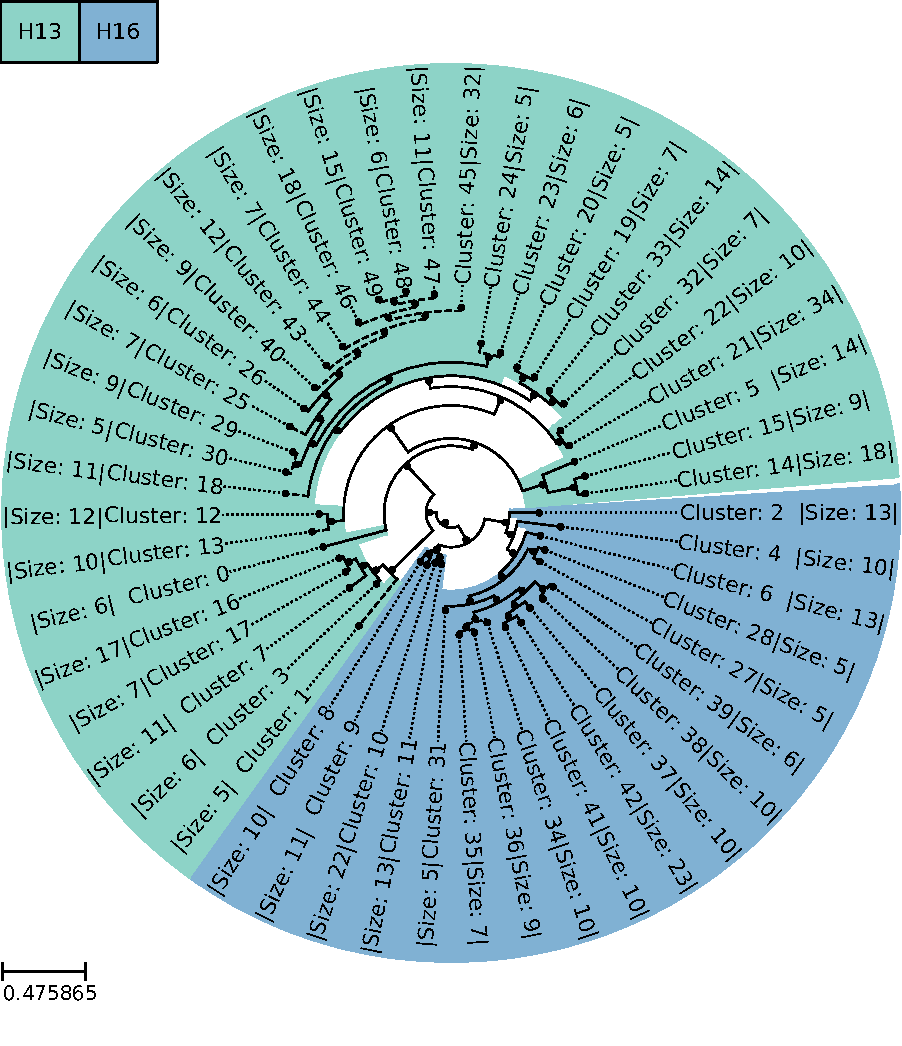
\includegraphics[width=\textwidth]{PCA/Clustertree_Segment_4_H_Cosine.pdf}
    \caption[Simple clustering tree of H13/H16 with cosine distance]{\textbf{Simple clustering tree of H13/H16 with cosine distance.} Cluster tree, based on the clustering by simple \texttt{HDBSCAN} without any $\varepsilon$ exploration and hybrid clustering. The matrix used contained precalculated cosine distances of all the k-mer frequency vectors to each other. The used vectors were calculated from the sequences, present in the H13 and H16 clusters in \autoref{fig:PCA_Clusteree_Knee_4} without reduction with \texttt{PCA} or \texttt{UMAP}. Therefore, \texttt{HDBSCAN} was used with precalculation input instead of a distance metric.}
    \label{fig:Simple_Clustertree_Cosine}
\end{figure}

\begin{figure}[!hbt]
    \centering
    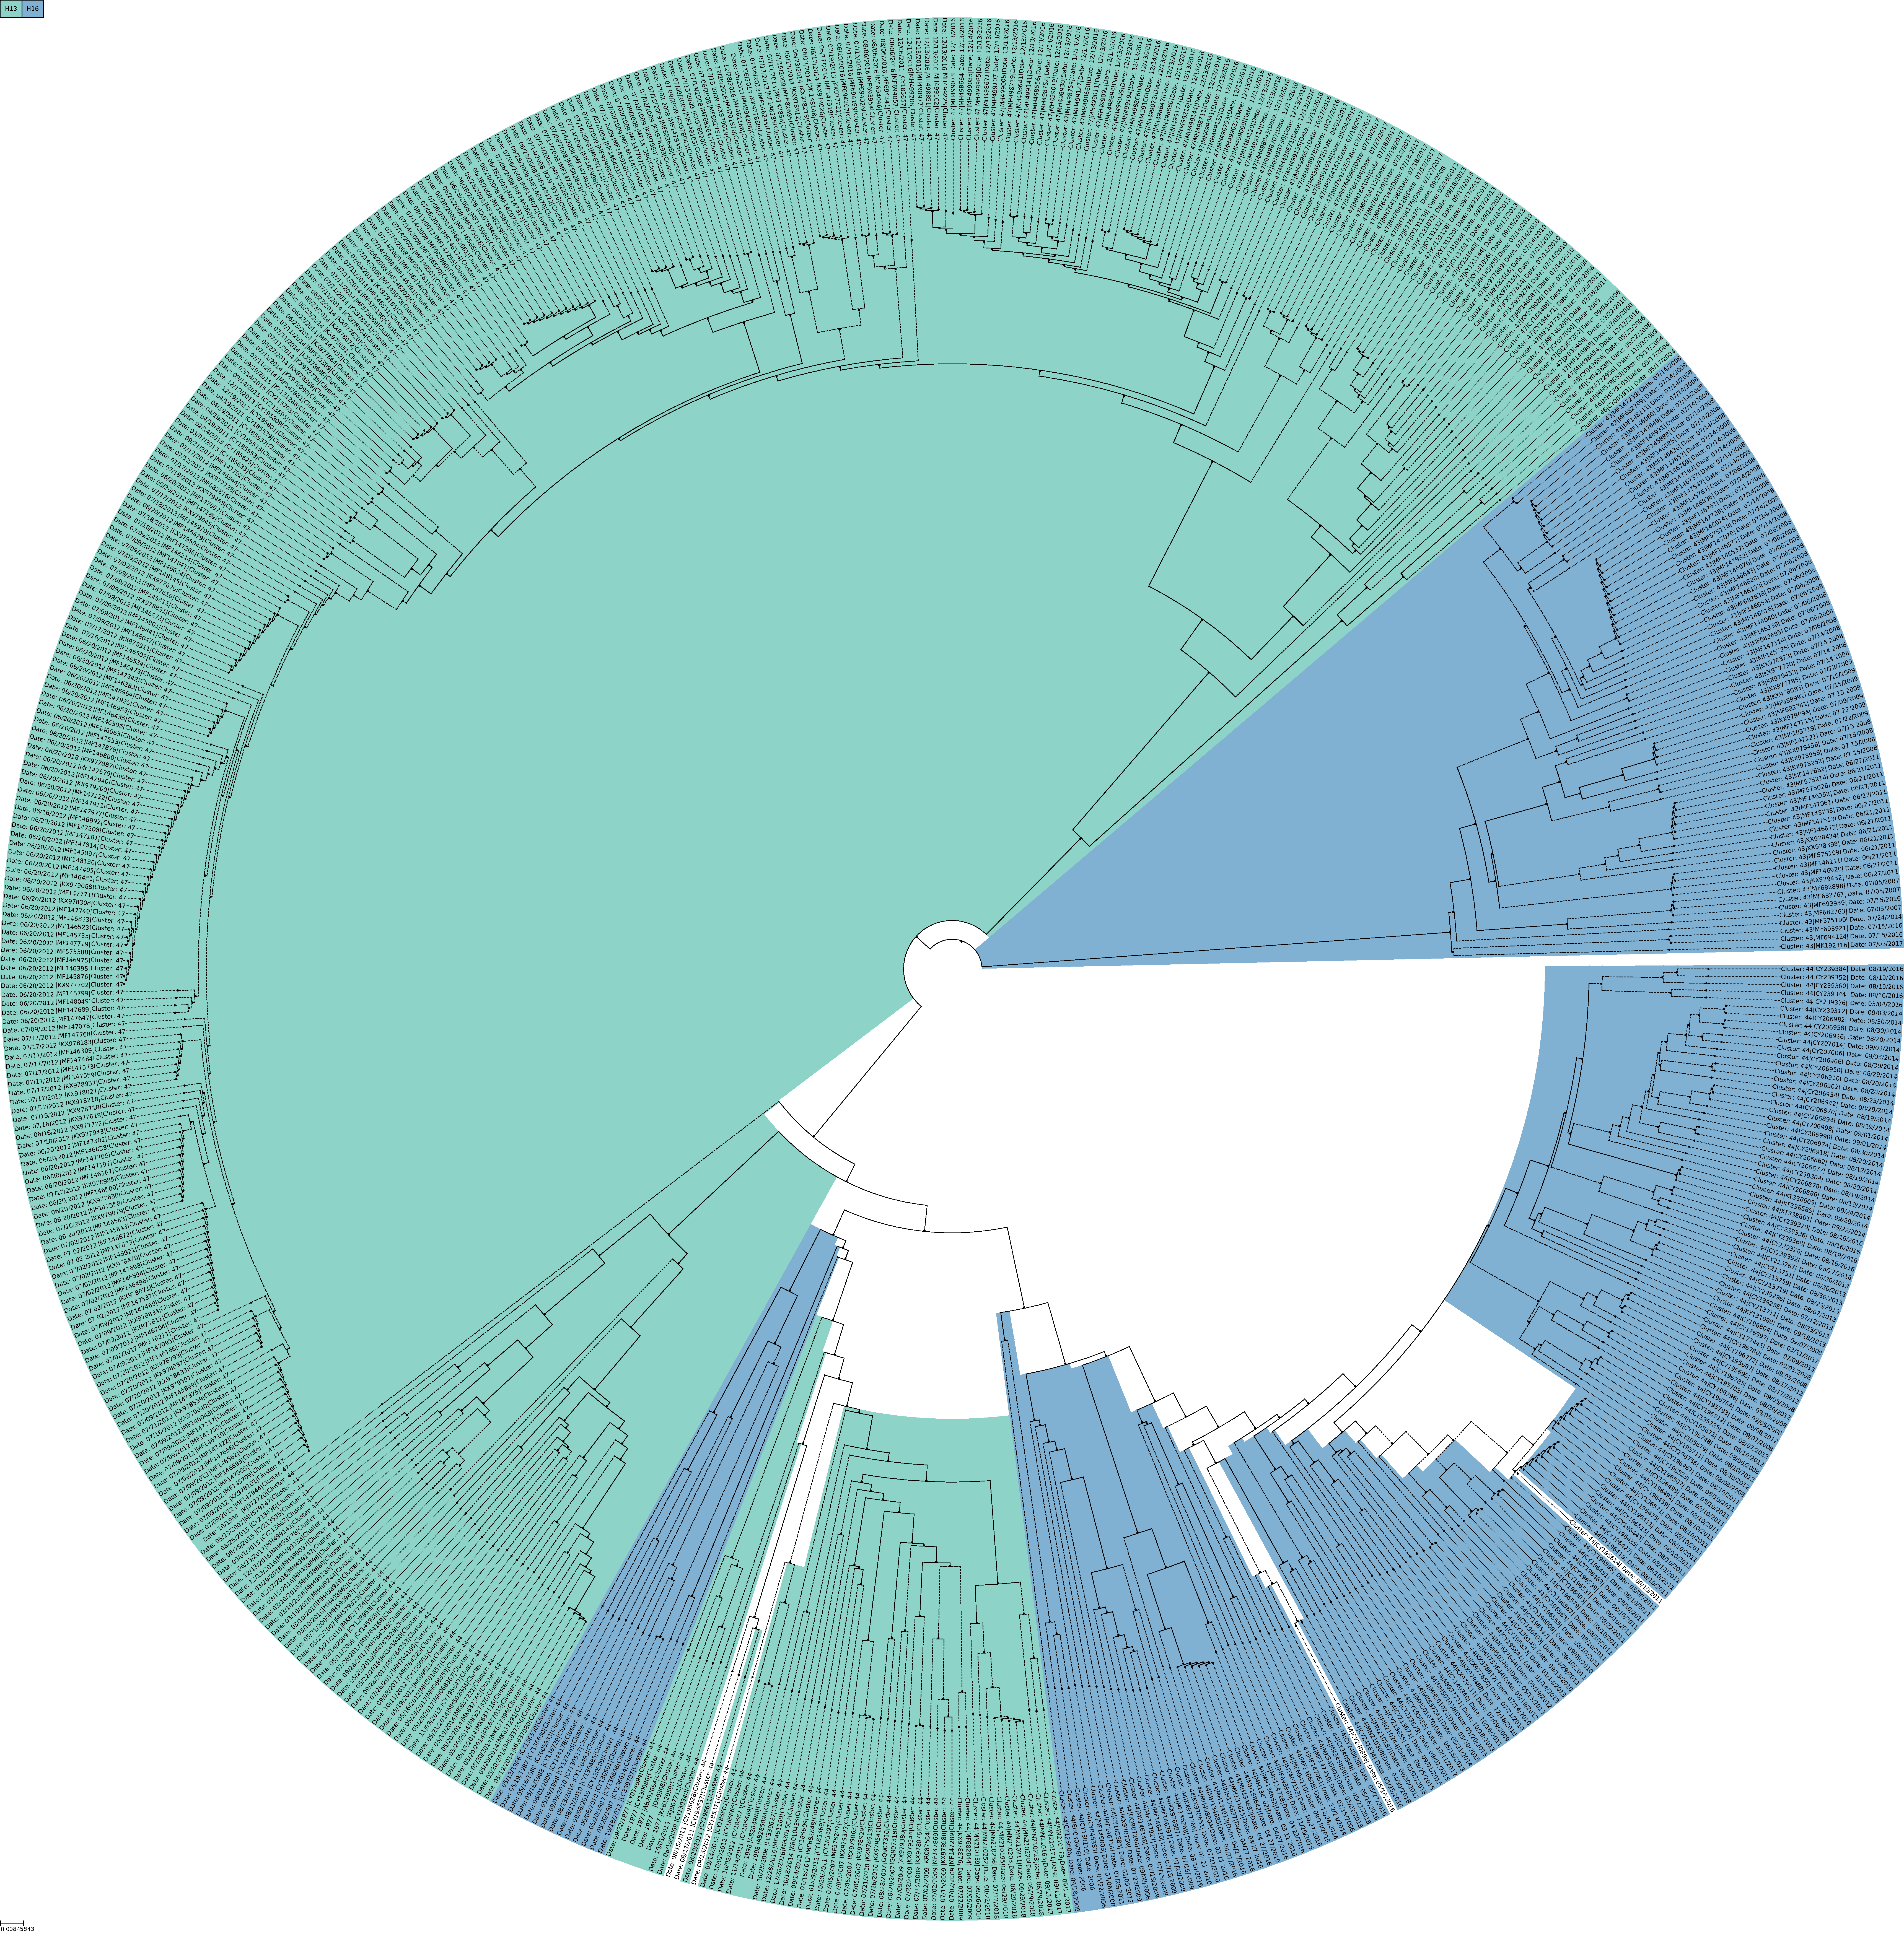
\includegraphics[width=\textwidth]{PCA/Clustertree_Segment_4_H_Focus.pdf}
    \caption[Simple clustering tree of H13/H16 with evolutionary distance]{\textbf{Simple clustering tree of H13/H16 with evolutionary distance.} Cluster tree, based on the clustering by simple \texttt{HDBSCAN} without any $\varepsilon$ exploration and hybrid clustering. The matrix used contained precalculated \gls{MSA} based distances of all the sequences to each other. The sequences, present in the H13 and H16 clusters in \autoref{fig:PCA_Clusteree_Knee_4} were used for the \gls{MSA}. Therefore, \texttt{HDBSCAN} was used with precalculation input instead of a distance metric.}
    \label{fig:Simple_Clustertree_MSA}
\end{figure}

\begin{figure}[!hbt]
    \centering
    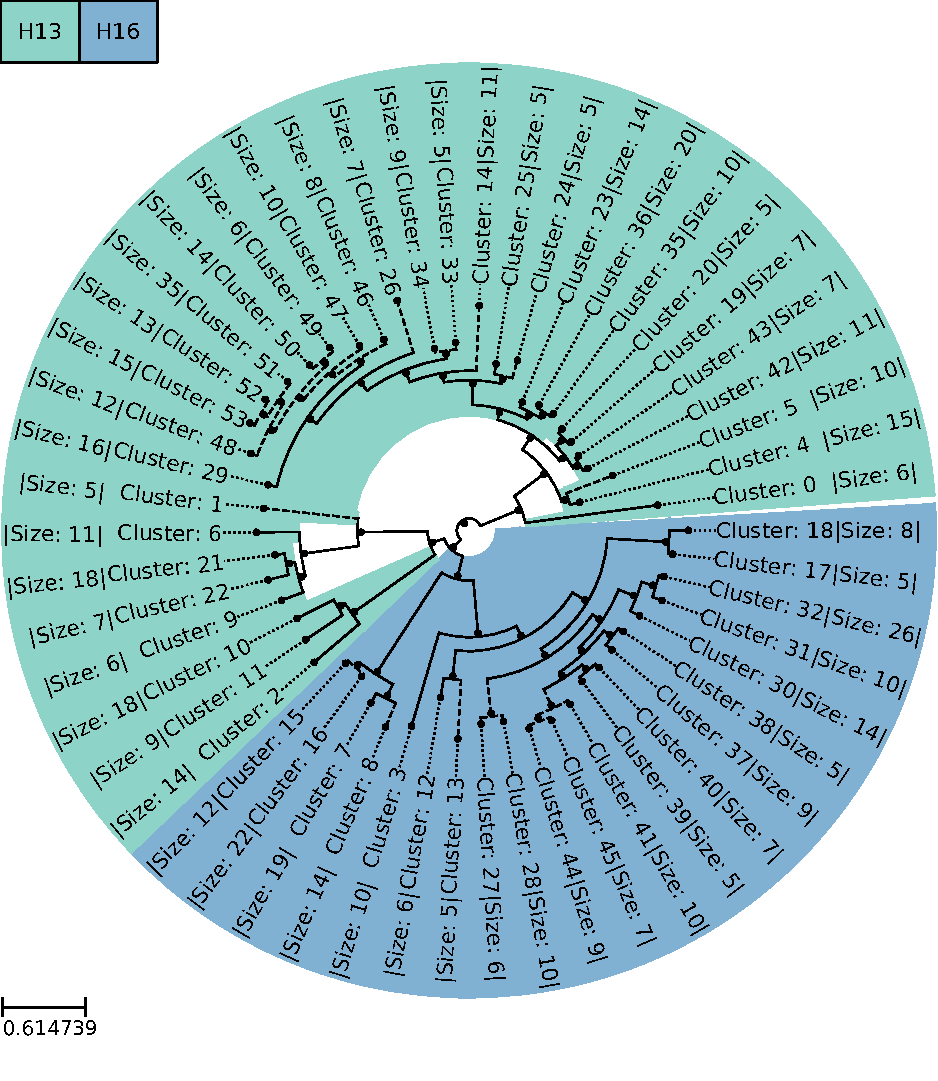
\includegraphics[width=\textwidth]{PCA/Clustertree_Segment_4_H_Simple.pdf}
    \caption[Simple clustering tree of H13/H16 with PCA]{\textbf{Simple clustering tree of H13/H16 with PCA.} Cluster tree, based on the clustering by simple \texttt{HDBSCAN} without any $\varepsilon$ exploration and hybrid clustering. The used vectors were calculated from the sequences, present in the H13 and H16 clusters in \autoref{fig:PCA_Clusteree_Knee_4} with prior \texttt{PCA} reduction to 30 dimensions.}
    \label{fig:Simple_Clustertree_PCA}
\end{figure}

In a similar manner to the precalculated \gls{UPGMA} tree in \autoref{fig:Precalculated_Cosine}, the subtypes are completely separated and split on both sides in two subgroups. This points to the fact, that the \texttt{HDBSCAN} clustering of the precalculated cosine distances of the k-mer frequencies are as usable as the k-mer frequencies itself and are able to draw a clear line to separate the subtypes. This finding is in line with the second cluster tree based on similar clustering on the same sequences with evolutionary distances of a \gls{MSA} instead (\autoref{fig:Alignment_Pipeline} pathway \textsf{\textbf{6}}). The same separation is even more obvious, as the subtypes sub trees are farther away from the separation at the trees root. On the side of the H13 sequences, a subdivision is also clearly noticeable. Subgroups in the H16 sequences are, on the other hand, not that clear separated in \autoref{fig:Simple_Clustertree_MSA}. Maybe the different distances between the subtypes and the subgroups on each side of the subtypes is different because evolutionary aspects like nucleotides that are more likely to change are involved in the \gls{MSA}. In the k-mer frequencies, the pure constellation of nucleotides is used, evolutionary aspects are neglected. Still, the precalculated approach as well as the \gls{MSA} evolutionary distances used the full information available from the sequences themselves, since no reduction with \texttt{PCA} or \texttt{UMAP} was performed and both indicate full subtype separation. Therefore these cluster trees (\autoref{fig:Simple_Clustertree_Cosine} and \autoref{fig:Simple_Clustertree_MSA}) are the only ground truth for H13/H16 clustering with \texttt{HDBSCAN} available. As already mentioned precalculated clustering with \texttt{HDBSCAN}, is a highly computationally expensive, as the matrices of size $n \times n$ have to be calculated and saved to be used in \texttt{HDBSCAN}. The calculation is, therefore, not possible without the availability of major RAM space. When using \texttt{HDBSCAN} with the k-mer vectors posterior to reduction with \texttt{PCA} to 30 dimensions, only a matrix of size $n\times 30$ has to be saved without the necessity of any distance precalculation. This is a \textbf{major} reduction of computational power necessary. A third clustering tree using reduced vectors on the same H13/H16 sequences should therefore represent the previous trees as best as possible. As described in \autoref{sec:Clustering} the method using \texttt{PCA} and the Kneedle Algorithm was declared as best method for \gls{IAV} clustering (PK). In the comparison by standard \texttt{HDBSCAN} clustering without $\varepsilon$ exploration, the sole reduction with \texttt{PCA}, representing simplified PK method should, match the ground truth (\autoref{fig:Simple_Clustertree_PCA}).

\vspace{1em}

Unfortunately, some major differences between the clustering trees using \texttt{PCA} and the two trees using precalculated cosine distance \gls{MSA} evolutionary distance stood out (\autoref{fig:Simple_Clustertree_Cosine}, \autoref{fig:Simple_Clustertree_MSA} and \autoref{fig:Simple_Clustertree_PCA}). The same clustering behavior as in the complete cluster tree in the previous section can be observed as no clear separation on the H13 and H16 clusters is present (\autoref{fig:Simple_Clustertree_PCA} and \autoref{fig:PCA_Clusteree_Knee_4} \textbf{\textsf{B}}). Since the distance calculation by \texttt{HDBSCAN} only used in the third tree is proportional to cosine precalculation (\autoref{fig:Reduction_Comparison}), the \texttt{PCA} or dimension reduction step seems to be the origin of the clustering error in \autoref{fig:PCA_Cluster_Knee_4} \textbf{\textsf{B}} and \textbf{\textsf{D}}. 

\vspace{1em}

As already mentioned, the precalculated cluster trees use the whole available amount of information given by the sequences. Either by direct use of the nucleotide comparisons with \gls{MSA} (\autoref{fig:Simple_Clustertree_MSA}) or by using the k-mer frequency vectors without reducing the dimension (\autoref{fig:Simple_Clustertree_Cosine}). Thus, the amount of information remaining in the vectors did not seem to suffice for the given task resulting in the differences in \autoref{fig:Simple_Clustertree_PCA}. The standard \texttt{HDBSCAN} clustering was also performed with the same subset of H13 and H16 sequences reduced with \texttt{UMAP} posterior to \texttt{PCA} (\autoref{fig:Simple_Clustertree_UMAP}) with results inferior to the sole use of \texttt{PCA}. In the appendix, a precalculated cluster tree using euclidean distance instead of cosine distance is also present, offering a similar result to the one using cosine distance (\autoref{fig:Simple_Clustertree_Euclid}).